\chapter{Anforderungsanalyse}
\label{sec:requirements}
% Wie ist die Ausgangslage (in Bamberg)? Wie werden/wurden die Anforderungen aufgestellt, 
% wer sind die Stakeholder und warum? Dann Anforderungen definieren und priorisieren
Bevor mit der eigentlichen Implementierung begonnen werden kann, ist es notwendig, die Anforderungsanalyse. Der erste Schritt hierzu besteht daraus, die Ausgangslage in Bamberg zu untersuchen, um darauf aufbauend die Stakeholder zu identifizieren, da diese den Ursprung der Anforderungen darstellen. Nachdem das Aufstellen der Anforderungen erfolgreich gewesen ist, können diese im Anschluss analysiert, also priorisiert, auf ihre Validität und im Anschluss auf ihre Realisierbarkeit überprüft werden. Basierend auf den Anforderungen werden dann Use Cases formuliert, die die Anforderungen in einer konkreten Situation beschreiben und damit die Grundlage für die Implementierung bilden.

\section{Ausgangslage in Bamberg}
\label{sec:ausgangslage}
Bamberg\sidenote{\url{https://www.stadt.bamberg.de/Unsere-Stadt/Stadtinfo/}} ist eine kreisfreie Stadt in Bayern im Regierungsbezirk Oberfranken mit einer Einwohnerzahl von knapp 80.000 Einwohnern (Stand: Dezember 2022). Die Stadt selbst kann dabei in sogenannte \ac{LCZ}, also Klassifikationen, welche sich durch die logische Aufteilung einer Landschaft ergeben \cite{stewart2011local}, unterteilt werden. Zusammen mit dem Domänenwissen des Meteorologen Prof.\ Dr.\ Thomas Foken (vgl. Kapitel \ref{sec:stakeholder}) hat eine rudimentäre Unterteilung in sechs \ac{LCZ} stattgefunden: Die Innenstadt, die ERBA, Gartenstadt, Bamberg-Ost, der Hain, am Laubanger und das Berggebiet (siehe Abbildung \ref{fig:lcz}). Die Entscheidung über die Grenzen und der Gebiete erfolgt dabei durch die in der Literatur gegebenen Charakteristika, welche zum Definieren von \ac{LCZ} notwendig sind \cite{oke2004initial, stewart2012local}:

\keyword{Innenstadt (2)} -- Die Innenstadt kann als \enquote{Compact midrise} klassifiziert werden. Charakteristisch für diese \ac{LCZ} ist der dichte Mix aus mittelhohen Gebäuden, das Vorhandensein von wenigen bis keinen Bäumen und hauptsächlich asphaltierten Landflächen. Überwiegend lassen sich Stein, Ziegel, Kacheln und Beton als Baumaterialien vorfinden.

\keyword{ERBA (6)} -- Die ERBA kann als \enquote{Open low-rise} klassifiziert werden. In einem solchen befinden sich in der Regel flache Gebäude, die in einer offeneren Struktur angeordnet sind. Die Landflächen sind asphaltiert, weisen aber auch Grünflächen in Form von kleinen Pflanzen oder verstreuten Bäumen auf. Die Baumaterialien sind ähnlich wie in der Innenstadt, jedoch kann man an der ERBA häufig Holz als Baumaterial vorfinden.

\keyword{Gartenstadt (6B)} -- Die Gartenstadt ist wie die ERBA ein \enquote{Open low-rise}. Allerdings kann hier der Zusatz \textit{\enquote{B}} als \enquote{Land cover type}\sidenote{Nach \cite{stewart2012local}: Klassifikationen zu saisonalen Eigenschaften, wie z.B. schneebedeckter Boden, trockener/feuchter Boden etc.} zur Klassifikation hinzugefügt werden, welche nach \cite{stewart2012local} bedeutet, dass die Landschaft rege mit immergrünen Bäumen bestückt ist. Die Landflächen weisen zu einem Großteil Grünflächen mit kleinen Pflanzen auf. Diese Arten von \ac{LCZ} werden in der Regel für Wälder oder Stadtparks verwendet.

\keyword{Bamberg-Ost (3)} -- Der Osten Bambergs wird als \enquote{Compact low-rise} klassifiziert. Dieser weist die identischen Charakteristika wie die Bamberger Innenstadt auf, mit dem einzigen Unterschied, dass es sich bei den Gebäuden um niedrige Gebäude handelt.

\keyword{Hain (5)} -- Der Hain befindet sich in der Klasse des \enquote{Open midrise}. Dieser weist die identischen Charakteristika wie die ERBA auf, mit dem einzigen Unterschied, dass es sich bei den Gebäuden um mittelhohe Gebäude handelt und statt Holz überwiegend Beton und Stahl als Baumaterialien eingesetzt werden.

\keyword{Laubanger (8)} -- Der Laubanger wird in Bamberg als \enquote{Large low-rise} eingestuft. In dieser Klasse lassen sich in der Regel große, aber flache Gebäude in einer offeneren Struktur vorfinden. Bäume oder Grünflächen sind meistens nicht bis kaum vorhanden, da die Straßen und Wege überwiegend asphaltiert sind. Als Baumaterialien kommen häufig Stahl, Beton und Stein zum Einsatz.

\keyword{Berggebiet (6A)} -- Das Bamberger Berggebiet ähnlich wie die Gartenstadt und ERBA als \enquote{Open low-rise} eingestuft und weist die identischen Charakteristika auf. Der Zusatz \textit{\enquote{A}} besagt hierbei, dass eine große bzw. dichte Menge an Bäumen in der Landschaft vorzufinden ist, was in der Regel auch für Wälder oder Stadtparks zutrifft.

\begin{figure}[t] % [t]: place at top of page (recommended)
    \centering
    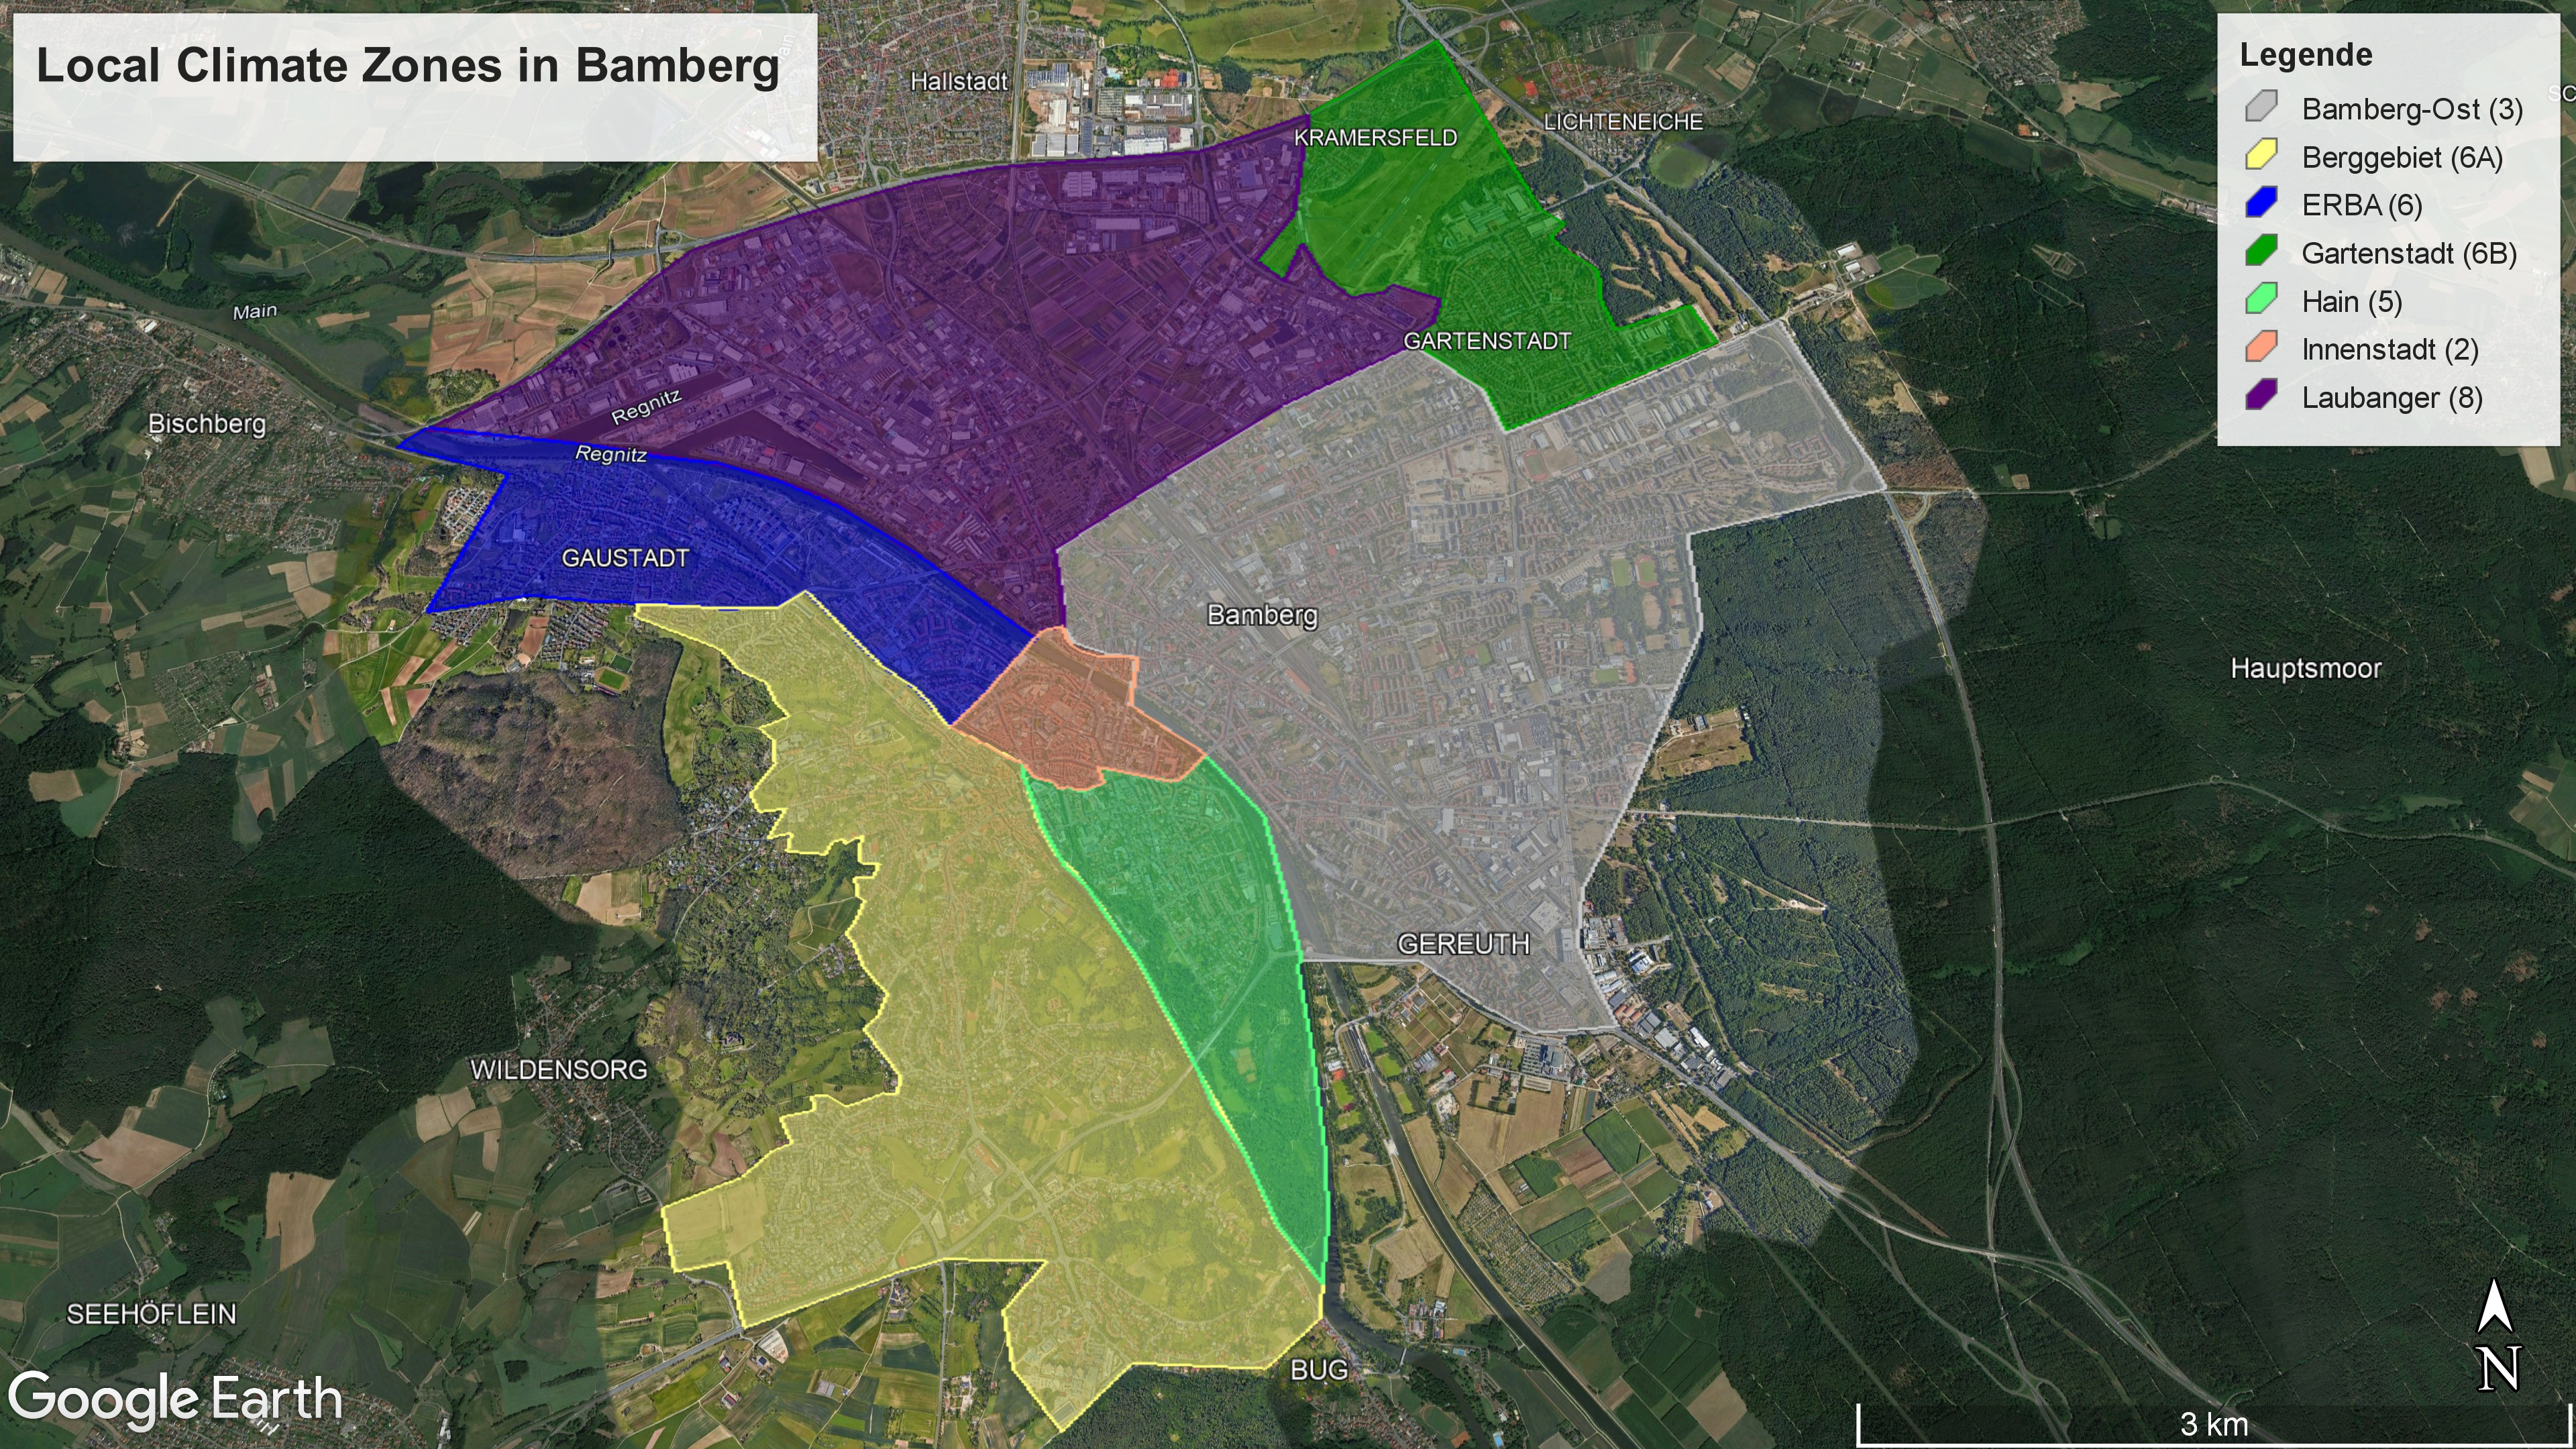
\includegraphics[width=1\textwidth]{figures/lcz.jpg}
    \decoRule
    \caption[LCZ in Bamberg]{Die sechs \ac{LCZ} in Bamberg (eigene Darstellung, basierend auf \cite{stewart2012local,oke2004initial})} 
    \label{fig:lcz}
\end{figure}

Durch die Unterteilung der Stadt Bamberg in \ac{LCZ} ist es möglich, die Auslesungen der Wetterstationen und die Unterschiede der Messwerte in den einzelnen Gebieten nachvollziehen und damit besser analysieren zu können. Der \ac{BVM} (vgl. Kapitel \ref{sec:stakeholder}) misst derzeit mithilfe von insgesamt 13 smarten Netatmo-Wetterstationen\sidenote{\url{https://shop.netatmo.com/de-de/weather/smart-weather-station/weatherstation}} (Stand: 21. Oktober 2023) verteilt in der gesamten Stadt die Temperatur und die Luftfeuchtigkeit an den entsprechenden Standorten\sidenote{Standorte der smarten Wetterstationen (LCZ): Steinertstraße (Innenstadt), Lange Straße (Innenstadt), Grünhundsbrunnen, Am Weidenufer, Holzmarkt (Innenstadt), Promenadestraße (Innenstadt), Obere Sandstraße (Innenstadt), Fischerei (Innenstadt), Wetzelstraße (ERBA), Ottostraße (Hain), Frauenstraße (Hain) (Innenstadt), Hainstraße (Hain), Schützenstraße (Hain) und in Bischberg (außerhalb der \ac{LCZ}, da Landkreis Bamberg, aber ERBA zuzuordnen)}. Aus den Messungen der Wetterstationen ergibt sich, dass sich die Bamberger Innenstadt im Vergleich zu anderen \ac{LCZ} kaum abkühlt und die Temperaturen sich häufig von der offiziellen Station des \ac{DWD} unterscheiden (vgl. Webauftritt\sidenote{\url{https://bvm-bamberg.de/de/projektseiten/klima/}} des Klimamessnetzes Bamberg). 
% hier jetzt die verschiedenen Stadtgebiete mit der Literatur beschreiben, dann sowas wie CO2-Emissionen der Stadt aufbringen, dann sowas wie "das meiste geht von der Innenstadt aus" kP

\subsection{Identifikation der Stakeholder}
\label{sec:stakeholder}

\paragraph{Der Bürgerverein Bamberg Mitte e.V.}

\paragraph{Die Domänenexperten} abc 123 test

\paragraph{Der Lehrstuhl für Informatik, insbesondere Mobile Softwaresysteme/Mobilität der Universität Bamberg}

\subsection{Das Bamberger Klimamessnetz als Grundlage der Sensordaten}

\section{Die Netatmo API --- eine Schnittstelle zwischen Sensordaten und Stakeholder}

\section{Definition der Anforderungen}

\section{Use Cases}